% Options for packages loaded elsewhere
\PassOptionsToPackage{unicode}{hyperref}
\PassOptionsToPackage{hyphens}{url}
\PassOptionsToPackage{dvipsnames,svgnames,x11names}{xcolor}
%
\documentclass[
  super,
  preprint,
  3p]{elsarticle}

\usepackage{amsmath,amssymb}
\usepackage{iftex}
\ifPDFTeX
  \usepackage[T1]{fontenc}
  \usepackage[utf8]{inputenc}
  \usepackage{textcomp} % provide euro and other symbols
\else % if luatex or xetex
  \usepackage{unicode-math}
  \defaultfontfeatures{Scale=MatchLowercase}
  \defaultfontfeatures[\rmfamily]{Ligatures=TeX,Scale=1}
\fi
\usepackage{lmodern}
\ifPDFTeX\else  
    % xetex/luatex font selection
\fi
% Use upquote if available, for straight quotes in verbatim environments
\IfFileExists{upquote.sty}{\usepackage{upquote}}{}
\IfFileExists{microtype.sty}{% use microtype if available
  \usepackage[]{microtype}
  \UseMicrotypeSet[protrusion]{basicmath} % disable protrusion for tt fonts
}{}
\makeatletter
\@ifundefined{KOMAClassName}{% if non-KOMA class
  \IfFileExists{parskip.sty}{%
    \usepackage{parskip}
  }{% else
    \setlength{\parindent}{0pt}
    \setlength{\parskip}{6pt plus 2pt minus 1pt}}
}{% if KOMA class
  \KOMAoptions{parskip=half}}
\makeatother
\usepackage{xcolor}
\setlength{\emergencystretch}{3em} % prevent overfull lines
\setcounter{secnumdepth}{5}
% Make \paragraph and \subparagraph free-standing
\ifx\paragraph\undefined\else
  \let\oldparagraph\paragraph
  \renewcommand{\paragraph}[1]{\oldparagraph{#1}\mbox{}}
\fi
\ifx\subparagraph\undefined\else
  \let\oldsubparagraph\subparagraph
  \renewcommand{\subparagraph}[1]{\oldsubparagraph{#1}\mbox{}}
\fi

\usepackage{color}
\usepackage{fancyvrb}
\newcommand{\VerbBar}{|}
\newcommand{\VERB}{\Verb[commandchars=\\\{\}]}
\DefineVerbatimEnvironment{Highlighting}{Verbatim}{commandchars=\\\{\}}
% Add ',fontsize=\small' for more characters per line
\usepackage{framed}
\definecolor{shadecolor}{RGB}{241,243,245}
\newenvironment{Shaded}{\begin{snugshade}}{\end{snugshade}}
\newcommand{\AlertTok}[1]{\textcolor[rgb]{0.68,0.00,0.00}{#1}}
\newcommand{\AnnotationTok}[1]{\textcolor[rgb]{0.37,0.37,0.37}{#1}}
\newcommand{\AttributeTok}[1]{\textcolor[rgb]{0.40,0.45,0.13}{#1}}
\newcommand{\BaseNTok}[1]{\textcolor[rgb]{0.68,0.00,0.00}{#1}}
\newcommand{\BuiltInTok}[1]{\textcolor[rgb]{0.00,0.23,0.31}{#1}}
\newcommand{\CharTok}[1]{\textcolor[rgb]{0.13,0.47,0.30}{#1}}
\newcommand{\CommentTok}[1]{\textcolor[rgb]{0.37,0.37,0.37}{#1}}
\newcommand{\CommentVarTok}[1]{\textcolor[rgb]{0.37,0.37,0.37}{\textit{#1}}}
\newcommand{\ConstantTok}[1]{\textcolor[rgb]{0.56,0.35,0.01}{#1}}
\newcommand{\ControlFlowTok}[1]{\textcolor[rgb]{0.00,0.23,0.31}{#1}}
\newcommand{\DataTypeTok}[1]{\textcolor[rgb]{0.68,0.00,0.00}{#1}}
\newcommand{\DecValTok}[1]{\textcolor[rgb]{0.68,0.00,0.00}{#1}}
\newcommand{\DocumentationTok}[1]{\textcolor[rgb]{0.37,0.37,0.37}{\textit{#1}}}
\newcommand{\ErrorTok}[1]{\textcolor[rgb]{0.68,0.00,0.00}{#1}}
\newcommand{\ExtensionTok}[1]{\textcolor[rgb]{0.00,0.23,0.31}{#1}}
\newcommand{\FloatTok}[1]{\textcolor[rgb]{0.68,0.00,0.00}{#1}}
\newcommand{\FunctionTok}[1]{\textcolor[rgb]{0.28,0.35,0.67}{#1}}
\newcommand{\ImportTok}[1]{\textcolor[rgb]{0.00,0.46,0.62}{#1}}
\newcommand{\InformationTok}[1]{\textcolor[rgb]{0.37,0.37,0.37}{#1}}
\newcommand{\KeywordTok}[1]{\textcolor[rgb]{0.00,0.23,0.31}{#1}}
\newcommand{\NormalTok}[1]{\textcolor[rgb]{0.00,0.23,0.31}{#1}}
\newcommand{\OperatorTok}[1]{\textcolor[rgb]{0.37,0.37,0.37}{#1}}
\newcommand{\OtherTok}[1]{\textcolor[rgb]{0.00,0.23,0.31}{#1}}
\newcommand{\PreprocessorTok}[1]{\textcolor[rgb]{0.68,0.00,0.00}{#1}}
\newcommand{\RegionMarkerTok}[1]{\textcolor[rgb]{0.00,0.23,0.31}{#1}}
\newcommand{\SpecialCharTok}[1]{\textcolor[rgb]{0.37,0.37,0.37}{#1}}
\newcommand{\SpecialStringTok}[1]{\textcolor[rgb]{0.13,0.47,0.30}{#1}}
\newcommand{\StringTok}[1]{\textcolor[rgb]{0.13,0.47,0.30}{#1}}
\newcommand{\VariableTok}[1]{\textcolor[rgb]{0.07,0.07,0.07}{#1}}
\newcommand{\VerbatimStringTok}[1]{\textcolor[rgb]{0.13,0.47,0.30}{#1}}
\newcommand{\WarningTok}[1]{\textcolor[rgb]{0.37,0.37,0.37}{\textit{#1}}}

\providecommand{\tightlist}{%
  \setlength{\itemsep}{0pt}\setlength{\parskip}{0pt}}\usepackage{longtable,booktabs,array}
\usepackage{calc} % for calculating minipage widths
% Correct order of tables after \paragraph or \subparagraph
\usepackage{etoolbox}
\makeatletter
\patchcmd\longtable{\par}{\if@noskipsec\mbox{}\fi\par}{}{}
\makeatother
% Allow footnotes in longtable head/foot
\IfFileExists{footnotehyper.sty}{\usepackage{footnotehyper}}{\usepackage{footnote}}
\makesavenoteenv{longtable}
\usepackage{graphicx}
\makeatletter
\def\maxwidth{\ifdim\Gin@nat@width>\linewidth\linewidth\else\Gin@nat@width\fi}
\def\maxheight{\ifdim\Gin@nat@height>\textheight\textheight\else\Gin@nat@height\fi}
\makeatother
% Scale images if necessary, so that they will not overflow the page
% margins by default, and it is still possible to overwrite the defaults
% using explicit options in \includegraphics[width, height, ...]{}
\setkeys{Gin}{width=\maxwidth,height=\maxheight,keepaspectratio}
% Set default figure placement to htbp
\makeatletter
\def\fps@figure{htbp}
\makeatother

\makeatletter
\makeatother
\makeatletter
\makeatother
\makeatletter
\@ifpackageloaded{caption}{}{\usepackage{caption}}
\AtBeginDocument{%
\ifdefined\contentsname
  \renewcommand*\contentsname{Table of contents}
\else
  \newcommand\contentsname{Table of contents}
\fi
\ifdefined\listfigurename
  \renewcommand*\listfigurename{List of Figures}
\else
  \newcommand\listfigurename{List of Figures}
\fi
\ifdefined\listtablename
  \renewcommand*\listtablename{List of Tables}
\else
  \newcommand\listtablename{List of Tables}
\fi
\ifdefined\figurename
  \renewcommand*\figurename{Figure}
\else
  \newcommand\figurename{Figure}
\fi
\ifdefined\tablename
  \renewcommand*\tablename{Table}
\else
  \newcommand\tablename{Table}
\fi
}
\@ifpackageloaded{float}{}{\usepackage{float}}
\floatstyle{ruled}
\@ifundefined{c@chapter}{\newfloat{codelisting}{h}{lop}}{\newfloat{codelisting}{h}{lop}[chapter]}
\floatname{codelisting}{Listing}
\newcommand*\listoflistings{\listof{codelisting}{List of Listings}}
\makeatother
\makeatletter
\@ifpackageloaded{caption}{}{\usepackage{caption}}
\@ifpackageloaded{subcaption}{}{\usepackage{subcaption}}
\makeatother
\makeatletter
\@ifpackageloaded{tcolorbox}{}{\usepackage[skins,breakable]{tcolorbox}}
\makeatother
\makeatletter
\@ifundefined{shadecolor}{\definecolor{shadecolor}{rgb}{.97, .97, .97}}
\makeatother
\makeatletter
\makeatother
\makeatletter
\makeatother
\journal{Journal Name}
\ifLuaTeX
  \usepackage{selnolig}  % disable illegal ligatures
\fi
\usepackage[]{natbib}
\bibliographystyle{elsarticle-num}
\IfFileExists{bookmark.sty}{\usepackage{bookmark}}{\usepackage{hyperref}}
\IfFileExists{xurl.sty}{\usepackage{xurl}}{} % add URL line breaks if available
\urlstyle{same} % disable monospaced font for URLs
\hypersetup{
  pdftitle={The Application of Machine Learning to Predict NFL Running Back Performance},
  pdfauthor={Giovanni Lunetta; Sam Lutzel},
  pdfkeywords={Machine Learning, Predictive Analytics, Sports
Analytics},
  colorlinks=true,
  linkcolor={blue},
  filecolor={Maroon},
  citecolor={Blue},
  urlcolor={Blue},
  pdfcreator={LaTeX via pandoc}}

\setlength{\parindent}{6pt}
\begin{document}

\begin{frontmatter}
\title{The Application of Machine Learning to Predict NFL Running Back
Performance \\\large{STATS-5405} }
\author[1]{Giovanni Lunetta%
\corref{cor1}%
}
 \ead{giovanni.lunetta@uconn.edu} 
\author[1]{Sam Lutzel%
\corref{cor1}%
}
 \ead{samuel.lutzel@uconn.edu} 

\affiliation[1]{organization={University of
Connecticut, Statistics},addressline={2075 Hillside
Road},city={Storrs},postcode={6269},postcodesep={}}

\cortext[cor1]{Corresponding author}


        
\begin{abstract}
This study employs an ensemble of machine learning techniques, including
Multiple Linear Regression (MLR), Generalized Linear Models (GLM), and
XGBoost to enhance predictive analytics in the National Football League
(NFL). The research focuses on one of the most critical aspects of
football offense - the running game. In order to predict the yards
gained by NFL running backs following a handoff, the study analyzes a
plethora of player tracking data from the 2017 to 2019 seasons. It
integrates a variety of factors such as player positions, orientation,
and the situational context of the game, including down, distance, and
field position. This multifaceted approach aims to yield highly accurate
models that can serve as valuable tools for coaching staffs to optimize
play-calling, manage player workloads, and enhance game planning. The
predictive insights derived from this research are intended to support
teams in deploying their running backs more effectively, leading to
potentially improved outcomes on the field. As the NFL continues to
evolve with a greater emphasis on analytics, this study seeks to
contribute significantly to the field of sports analytics by providing a
model that underscores the importance of the running game in a
predominantly pass-oriented league.
\end{abstract}





\begin{keyword}
    Machine Learning \sep Predictive Analytics \sep 
    Sports Analytics
\end{keyword}
\end{frontmatter}
    \ifdefined\Shaded\renewenvironment{Shaded}{\begin{tcolorbox}[frame hidden, enhanced, borderline west={3pt}{0pt}{shadecolor}, boxrule=0pt, sharp corners, interior hidden, breakable]}{\end{tcolorbox}}\fi

\hypertarget{introduction}{%
\section{Introduction}\label{introduction}}

\hypertarget{background-of-the-national-football-league}{%
\subsection{Background of the National Football
League}\label{background-of-the-national-football-league}}

The National Football League (NFL) is the most popular professional
sports league in the United States, with an estimated 187 million fans.
The league consists of 32 teams divided into two conferences, the
American Football Conference (AFC) and the National Football Conference
(NFC). Each conference is further divided into four divisions, with four
teams in each division. The NFL season consists of 17 weeks, with each
team playing 16 games and having one bye week. The regular season is
followed by a 12-team playoff, with the winner of each conference
advancing to the Super Bowl, the league's championship game.

The NFL game strategy primarily consists of two ways to advance the
football down the field: running and passing. Running the ball is
defined as a play in which the quarterback gives the ball to another
player that is located behind them (a handoff or a small toss). The
player then attempts to run the ball down the field as far as possible
before being tackled to the ground. Passing the ball is defined as a
play in which the quarterback throws the ball to another player down the
field. The player then attempts to catch the ball and advance it down
the field as far as possible before being tackled to the ground. The
goal of each team is to score as many points as possible by advancing
the ball down the field and into the end zone or by kicking the ball
through the field goal posts. The team with the most points at the end
of the game wins.

\hypertarget{motivation}{%
\subsection{Motivation}\label{motivation}}

The primary goal of this research is to develop cutting-edge predictive
models capable of accurately estimating the yards a running back will
gain after a handoff during NFL games. This objective is pivotal for
formulating advanced offensive strategies and refining player
evaluations. The running play is a fundamental aspect of the game that
can dictate the tempo, control the clock, and establish physical
dominance.

The motivation behind this study stems from the transformative impact
that data analytics has had on sports, particularly in the NFL, where
the fusion of technology and sports science has begun to redefine how
the game is played and understood. In an era where marginal gains are
increasingly sought after, the ability to predict the outcome of running
plays with high precision can provide teams with a significant
competitive advantage. It enables coaches to make informed decisions
regarding play selection, player rotations, and game management,
especially in critical moments of a match. Additionally, the insights
from this study can empower front offices in their scouting and drafting
processes by quantifying the expected value a running back adds to their
team. Furthermore, there is also a tremendous opportunity to leverage
these predictive models on the defensive end of the ball, allowing teams
to better anticipate and defend against running plays. With better
insights into the opponents running game, defenses can adjust their
schemes and personnel to counter the opposing team's offensive strategy,
such as by stacking the box or blitzing the quarterback. In addition to
the benefits performance analytics provides to the teams, it also helps
fans select better fantasy football teams and make more informed betting
decisions. This leads to a more engaging and enjoyable experience for
the fans, which is critical for the long-term success of the league.

Ultimately, the true beauty of this research lies in its ability to
bridge the gap between complex player tracking data and practical
on-field strategies. In specific, it's about enhancing the very essence
of the game and enriching the broader discourse on sports performance
analytics. By pioneering research in this domain, this study is set to
propel the analytical capabilities of NFL teams to new heights,
providing them with tools that were once considered unimaginable.
Ultimately, it contributes to the ongoing evolution of the sport itself,
marking a pivotal moment in the history of football and the broader
world of sports analytics.

\hypertarget{methods}{%
\section{Methods}\label{methods}}

\hypertarget{data-cleaning-and-preprocessing}{%
\subsection{Data Cleaning and
Preprocessing}\label{data-cleaning-and-preprocessing}}

Data cleaning and preprocessing are critical to ensuring the quality and
integrity of machine learning models. The cleaned dataset was obtained
by addressing any inconsistencies and handling missing data through
imputation techniques. Preprocessing steps included encoding categorical
variables using one-hot encoding or label encoding methods and scaling
and normalizing numerical variables to ensure they are on comparable
scales.

To begin, several variables were removed in order to simulate the
beginning of each play. For instance, the dataset include the speed,
acceleration, direction, and distance traveled of each player on the
field at the beginning of each play. However, this information is not
available to the coaching staff prior to the snap of the ball.
Therefore, these variables were removed from the datset. Furthermore,
some variables may introduce multicollinearity issues since they
represent the same information. For instance, the dataset includes the
name and id of each player on the field. However, these variables are
highly correlated with each other. Therefore, only one of these
variables was kept in the dataset.

When the dataset was first obtained, each row represented a single
player on the field. However, the goal of this study is to predict the
yards gained after a handoff for each play. Therefore, every 22 rows had
to be merged into one row (11 players on each side). During this
process, any duplicated information/columns were dropped from the
dataset. One example of this is the weather during the play. When all 22
rows are merged, it included the weather 22 times, even though weather
is only needed once.

In addition to the attempt at removing unnecessary variables and
proactively removing potenital multicollienarity issues, variables such
as weather, wind speed, and wind direction had multiple levels, some of
which represented the same data. For instance, ``rainy'' and ``showers''
were considered the same weather type. There were multiple instances of
relationships between inputs on the same variable that existed similar
to the example above. Due to this, these weather types were grouped into
one category - ``rain.'' This helps to drastically reduce the complexity
of the dataset. These variables were also converted to factors for the
modeling process.

Variables such as offense personnel had to be converted to dummy
variables. The input for each dummy variable was either 0 or 1 depending
on whether or not the offense had that personnel on the field. For
instance, if the offense had 2 running backs on the field, the input for
the ``RB'' dummy variable would be 2. The input for the ``WR'' dummy
variable would be 0 since there were no wide receivers on the field.
This process was repeated for all personnel types.

One additional step that was taken was the randomization of all plays
within the dataset. The reason for this randomization is to ensure that
each row (play of a game) is independent of one another. Furthermore,
the dataset only contains running plays. Therefore, passing plays that
occured between the running plays were removed. In other words, all
plays are not dependent on the previous outcome. In all, the
randomization of the dataset in conjunction with the removal of passing
plays ensures that each row is independent of one another.

\hypertarget{data-exploration}{%
\subsection{Data Exploration}\label{data-exploration}}

Prior to the development of the predictive models, a comprehensive
exploratory data analysis (EDA) was conducted to understand the
underlying structure and characteristics of the data. This step involved
visualizing the distribution of key variables, identifying patterns and
outliers, and exploring correlations and interactions between
predictors. Data visualization, through techniques like scatter plots,
histograms, and heatmaps, can offer an intuitive understanding of data
distributions, correlations, and potential clusters within the dataset.
EDA-informed feature selection and engineering strategies highlighted
potential predictors that are most informative of yards gained after a
handoff.

\hypertarget{feature-engineering}{%
\subsection{Feature Engineering}\label{feature-engineering}}

During preprocessing, we will also undertake feature engineering to
create new variables that may have a stronger relationship with the
target variable. This could include interaction terms that capture the
combined effect of two predictors, polynomial features for capturing
non-linear relationships, and domain-specific features that encapsulate
strategic elements of the game.

\hypertarget{model-development-and-evaluation}{%
\subsection{Model Development and
Evaluation}\label{model-development-and-evaluation}}

With a clean and prepared dataset, we will then proceed to develop our
MLR, GLM, and XGBoost models.

\hypertarget{multiple-linear-regression-mlr}{%
\subsection{Multiple Linear Regression
(MLR)}\label{multiple-linear-regression-mlr}}

Multiple linear regression models predict a continuous repsonse variable
using a linear combination of predictors. For our baseline MLR model, we
will use the ordinary least squares (OLS) method to estimate the
coefficients of our predictor variables. The model is specified as:

\(Y_i = \beta_0 + \beta_1X_{i1} + \beta_2X_{i2} + \ldots + \beta_jX_{ij} + \epsilon_i\)

where \(Y_i\) represents the yards gained after the handoff for the
\(i^{th}\) observation, \(X_{ij}\) is the \(i^{th}\) observation on the
\(j^{th}\) predictor variable (where \(j = 1, ..., p\)),~\(\beta_j\) is
the \(j^{th}\) coefficient to be estimated corresponding to the proper
\(X_{ij}\) variable, and \(\epsilon_i\) is the error term. The
\(j^{th}\) coefficient, \(\beta_j\), represents the change in the
response variable for a unit change in the \(X_{ij}\) predictor
variable, while holding all other predictors constant.

The ordinary least squares (OLS) method will be deployed to minimize the
sum of the squared differences between the observed and predicted
values. The optimization problem can be represented as minimizing the
sum of errors squared:

\[
\Sigma_{i=0}^n \epsilon_i^2 = \Sigma_{i=0}^n (Y_i - \hat{Y}_i)^2 = \Sigma_{i=0}^n (Y_i - \beta_0 - \beta_1X_{i1} - \ldots - \beta_jX_{ij})^2
\]

Here, \(\Sigma_{i=0}^n \epsilon_i^2\) represents the sum of the squared
residuals, which we aim to minimize. The variable \(\hat{Y}_i\)
represents the predicted outcome of the model for the \(i^{th}\)
observation. This approach assumes that the relationship between the
independent variables and the dependent variable is linear. To ensure
the robustness of our model, we will conduct a series of diagnostic
tests:

\begin{enumerate}
\def\labelenumi{\arabic{enumi}.}
\tightlist
\item
  Linearity: We will use scatter plots and residual plots to verify that
  the relationship between the predictors and the response is linear.
\item
  Homoscedasticity: We will inspect the residuals to confirm constant
  variance across all levels of the independent variables. This can be
  assessed visually using a residual vs.~fitted values plot.
\item
  Independence: The Durbin-Watson test will help in detecting the
  presence of autocorrelation in the residuals, which should not be
  present in the data.
\item
  Normality of Residuals: Normality will be checked using Q-Q plots and
  statistical tests like the Shapiro-Wilk test.
\end{enumerate}

If any assumptions are violated, we may consider transformations of
variables or the use of robust regression techniques.

\hypertarget{generalized-linear-models-glm}{%
\subsection{Generalized Linear Models
(GLM)}\label{generalized-linear-models-glm}}

GLMs extend the linear model framework to allow for response variables
that have error distribution models other than a normal distribution.
They are particularly useful when dealing with non-normal response
variables, such as count data or binary outcomes. In its general form, a
GLM consists of three elements:

\begin{enumerate}
\def\labelenumi{\arabic{enumi}.}
\tightlist
\item
  Random Component: Specifies the probability distribution of the
  response variable \(Y\), such as normal, binomial, Poisson, or
  exponential.
\item
  Systematic Component: A linear predictor \(\eta = X\beta\).
\item
  Link Function: A function \(g\) that relates the mean of the response
  variable \(E(Y)\) to the linear predictor \(\eta\).
\end{enumerate}

The choice of link function is crucial and is typically selected based
on the nature of the distribution of the response variable. For
instance, a logit link function is used for a binomial distribution, and
a log link function is often used for a Poisson distribution.

The likelihood function for a GLM can be written as:

\[
L(\beta) = \prod_{i=1}^{n} f(y_i; \theta_i, \phi)
\]

where \(f(y_i; \theta_i, \phi)\) is the probability function for the
\(i\)-th observation, \(\theta_i\) is the parameter of interest (e.g.,
mean), and \(\phi\) is the dispersion parameter. The goal is to find the
values of \(\beta\) that maximize this likelihood function.

\hypertarget{xgboost}{%
\subsection{XGBoost}\label{xgboost}}

XGBoost stands for eXtreme Gradient Boosting and is a
decision-tree-based ensemble Machine Learning algorithm that uses a
gradient boosting framework. It is a powerful technique that can handle
a variety of regression and classification problems. For regression, it
can be configured to optimize for different loss functions; the most
common for regression being the squared error loss:

\[
L(\theta) = \sum_{i=1}^{n}(y_i - \hat{y}_i)^2
\]

where \(y_i\) are the observed values, and \(\hat{y}_i\) are the
predicted values.

In XGBoost, each new tree is built to correct the errors made by the
previous ones. The algorithm combines weak predictive models to form a
strong predictor. The model's complexity is controlled by the
regularization term \(\Omega(\theta)\) which is a function of the tree
structure and the number of leaves. The overall objective function to be
minimized is:

\[
\text{Obj}(\theta) = L(\theta) + \lambda \sum_{k}(w_k^2) + \gamma T
\]

where \(w_k\) represents the leaf weights of the trees, \(T\) is the
number of leaves, \(\lambda\) is the L2 regularization term on the
weights, and \(\gamma\) is the complexity control on the number of
leaves. For regression tasks, we can also utilize the quantile loss
which is particularly useful for prediction intervals:

\[
L_{\tau}(\theta) = \sum_{i=1}^{n} \left[ \tau (y_i - \hat{y}_i) \mathbb{1}_{y_i \geq \hat{y}_i} + (1 - \tau) (\hat{y}_i - y_i) \mathbb{1}_{y_i < \hat{y}_i} \right]
\]

Here, 1 is an indicator function, and \(\tau\) is the quantile of
interest, allowing us to model different parts of the conditional
distribution of the response variable.

XGBoost also provides a feature importance score, which is a metric that
quantifies the contribution of each feature to the model's predictive
power. This is done by measuring the impact on the model's accuracy each
time a feature is used to split the data across all trees.

\hypertarget{model-performance-metrics}{%
\subsection{Model Performance Metrics}\label{model-performance-metrics}}

For MLR and GLM, the model's performance will be evaluated using metrics
such as the Mean Squared Error (MSE) and the Mean Absolute Error (MAE).
For the XGBoost model, along with MSE and MAE, we will assess
performance using additional metrics like the R-squared for regression
tasks and feature importance scores to understand which variables are
most predictive.

\hypertarget{model-interpretation-and-application}{%
\subsection{Model Interpretation and
Application}\label{model-interpretation-and-application}}

The final step will be to interpret the models in the context of NFL
games. This will involve translating the statistical outputs into
actionable insights for coaches and team strategists, providing
recommendations on how to leverage the results for competitive advantage
in play-calling and player evaluation.

\hypertarget{software-and-tools}{%
\subsection{Software and Tools}\label{software-and-tools}}

All analyses will be conducted in R, a statistical computing language
that provides a wide array of packages for machine learning and data
analysis. For MLR and GLM, we will utilize the \texttt{stats} package
that comes with the R base installation. For our XGBoost model, we will
use the \texttt{xgboost} package, which is specifically designed for
speed and performance. Data manipulation and cleansing will be managed
with packages like \texttt{dplyr} and \texttt{tidyr}, while
\texttt{ggplot2} will be employed for data visualization to facilitate
understanding and interpretation of the data and model outputs. For
feature engineering and preprocessing, we will take advantage of
\texttt{caret} or \texttt{recipes}. Hyperparameter tuning can be
optimized using the \texttt{tune} package, and for cross-validation, the
\texttt{rsample} package will be employed. The \texttt{broom} and
\texttt{modelr} packages will be useful for tidying model outputs and
working with models in a pipeline, respectively. This suite of packages
will enable a comprehensive workflow within R for developing,
evaluating, and interpreting the predictive models.

\hypertarget{multiple-linear-regression-model}{%
\section{Multiple Linear Regression
Model}\label{multiple-linear-regression-model}}

\hypertarget{model-development}{%
\subsection{Model Development}\label{model-development}}

First, lets start by importing the completely clean and ready to use
dataset. This dataset was the result of procedures outlined in the data
cleaning and preprocessing section.

\begin{Shaded}
\begin{Highlighting}[]
\CommentTok{\# Import the dataset}
\NormalTok{football\_data }\OtherTok{\textless{}{-}} \FunctionTok{read.csv}\NormalTok{(}\StringTok{"/Users/samlutz10/Desktop/STAT5405/Final Project/train\_ready.csv"}\NormalTok{)}
\end{Highlighting}
\end{Shaded}

Now that the data has been imported, splitting the data into a training
set and a testing set can commence. The training set will be used to
train the model, while the testing set will be used to test the model.
The training set will be 80\% of the data, while the testing set will be
20\% of the data.

\begin{Shaded}
\begin{Highlighting}[]
\CommentTok{\# Split the data into a training set and a testing set}
\FunctionTok{set.seed}\NormalTok{(}\DecValTok{123457}\NormalTok{)}
\NormalTok{train.prop }\OtherTok{\textless{}{-}} \FloatTok{0.80}
\NormalTok{strats }\OtherTok{\textless{}{-}}\NormalTok{ football\_data}\SpecialCharTok{$}\NormalTok{Yards}
\NormalTok{rr }\OtherTok{\textless{}{-}} \FunctionTok{split}\NormalTok{(}\DecValTok{1}\SpecialCharTok{:}\FunctionTok{length}\NormalTok{(strats), strats)}
\NormalTok{idx }\OtherTok{\textless{}{-}} \FunctionTok{sort}\NormalTok{(}\FunctionTok{as.numeric}\NormalTok{(}\FunctionTok{unlist}\NormalTok{(}\FunctionTok{sapply}\NormalTok{(rr, }
        \ControlFlowTok{function}\NormalTok{(x) }\FunctionTok{sample}\NormalTok{(x, }\FunctionTok{length}\NormalTok{(x)}\SpecialCharTok{*}\NormalTok{train.prop)))))}
\NormalTok{train.set }\OtherTok{\textless{}{-}}\NormalTok{ football\_data[idx, ]}
\NormalTok{test.set }\OtherTok{\textless{}{-}}\NormalTok{ football\_data[}\SpecialCharTok{{-}}\NormalTok{idx, ]}
\end{Highlighting}
\end{Shaded}

The average of yards in both the trainign and testing sets are computed
to ensure they are about the same. In addition, both of those should be
similar to that of the original dataset. This process will help to
ensure that the training and testing sets are representative of the
entire dataset.

The average of yards in both the trainign and testing sets are computed
to ensure they are about the same. In addition, both of those should be
similar to that of the original dataset. This process will help to
ensure that the training and testing sets are representative of the
entire dataset.

\begin{Shaded}
\begin{Highlighting}[]
\CommentTok{\# Check that the average of yards is about the same in both the training and testing sets}
\NormalTok{(ave\_train }\OtherTok{\textless{}{-}} \FunctionTok{mean}\NormalTok{(train.set}\SpecialCharTok{$}\NormalTok{Yards))}
\end{Highlighting}
\end{Shaded}

\begin{verbatim}
[1] 4.151264
\end{verbatim}

\begin{Shaded}
\begin{Highlighting}[]
\NormalTok{(ave\_test }\OtherTok{\textless{}{-}} \FunctionTok{mean}\NormalTok{(test.set}\SpecialCharTok{$}\NormalTok{Yards))}
\end{Highlighting}
\end{Shaded}

\begin{verbatim}
[1] 4.530165
\end{verbatim}

\begin{Shaded}
\begin{Highlighting}[]
\NormalTok{(ave\_all }\OtherTok{\textless{}{-}} \FunctionTok{mean}\NormalTok{(football\_data}\SpecialCharTok{$}\NormalTok{Yards))}
\end{Highlighting}
\end{Shaded}

\begin{verbatim}
[1] 4.227626
\end{verbatim}

Based on the results above, the average of yards is about the same in
both the training and testing sets. In addition, both of those are
similar to that of the original dataset.

Now that the data has been split into a training set and a testing set,
development of the model can begin.

The first model that will be synthesized has only an intercept and no
predictors.

\begin{Shaded}
\begin{Highlighting}[]
\NormalTok{lm\_model\_null }\OtherTok{\textless{}{-}} \FunctionTok{lm}\NormalTok{(Yards }\SpecialCharTok{\textasciitilde{}} \DecValTok{1}\NormalTok{, }\AttributeTok{data =}\NormalTok{ train.set)}
\FunctionTok{summary}\NormalTok{(lm\_model\_null)}
\end{Highlighting}
\end{Shaded}

\begin{verbatim}

Call:
lm(formula = Yards ~ 1, data = train.set)

Residuals:
    Min      1Q  Median      3Q     Max 
-16.151  -3.151  -1.151   1.849  85.849 

Coefficients:
            Estimate Std. Error t value Pr(>|t|)    
(Intercept)  4.15126    0.03843     108   <2e-16 ***
---
Signif. codes:  0 '***' 0.001 '**' 0.01 '*' 0.05 '.' 0.1 ' ' 1

Residual standard error: 6.047 on 24757 degrees of freedom
\end{verbatim}

\begin{Shaded}
\begin{Highlighting}[]
\CommentTok{\# Fit the model}
\NormalTok{lm\_model\_full }\OtherTok{\textless{}{-}} \FunctionTok{lm}\NormalTok{(Yards }\SpecialCharTok{\textasciitilde{}}\NormalTok{ ., }\AttributeTok{data =}\NormalTok{ train.set)}
\FunctionTok{summary}\NormalTok{(lm\_model\_full)}
\end{Highlighting}
\end{Shaded}

\begin{verbatim}

Call:
lm(formula = Yards ~ ., data = train.set)

Residuals:
    Min      1Q  Median      3Q     Max 
-17.608  -3.115  -1.115   1.415  87.578 

Coefficients:
                             Estimate Std. Error t value Pr(>|t|)    
(Intercept)                 3.208e+00  1.365e+01   0.235  0.81415    
XA0                         2.115e-03  1.026e-02   0.206  0.83665    
XA1                         6.044e-04  9.994e-03   0.060  0.95178    
XA2                         1.416e-03  1.013e-02   0.140  0.88882    
XA3                         1.334e-03  1.010e-02   0.132  0.89488    
XA4                        -1.413e-03  1.005e-02  -0.141  0.88810    
XA5                         2.272e-02  1.018e-02   2.231  0.02568 *  
XA6                         3.460e-03  1.029e-02   0.336  0.73667    
XA7                         5.608e-03  1.030e-02   0.545  0.58599    
XA8                        -8.735e-03  9.910e-03  -0.881  0.37812    
XA9                        -9.963e-03  1.009e-02  -0.988  0.32324    
XA10                       -1.672e-02  9.481e-03  -1.763  0.07788 .  
XB0                        -4.288e-03  1.025e-02  -0.418  0.67563    
XB1                        -1.614e-02  1.000e-02  -1.613  0.10667    
XB2                         5.075e-03  1.023e-02   0.496  0.61974    
XB3                         1.889e-02  1.011e-02   1.869  0.06169 .  
XB4                        -8.184e-03  1.004e-02  -0.815  0.41501    
XB5                        -6.650e-03  1.026e-02  -0.648  0.51674    
XB6                         2.272e-03  1.031e-02   0.220  0.82565    
XB7                        -9.978e-03  1.029e-02  -0.969  0.33234    
XB8                        -8.868e-04  9.904e-03  -0.090  0.92865    
XB9                         7.402e-03  1.009e-02   0.733  0.46337    
XB10                        1.180e-02  9.417e-03   1.253  0.21007    
YA0                         1.894e-03  5.676e-03   0.334  0.73858    
YA1                        -1.166e-02  5.695e-03  -2.048  0.04055 *  
YA2                         3.674e-03  5.565e-03   0.660  0.50907    
YA3                        -3.573e-03  5.465e-03  -0.654  0.51328    
YA4                        -8.558e-03  5.501e-03  -1.556  0.11977    
YA5                        -4.311e-04  5.535e-03  -0.078  0.93793    
YA6                        -1.715e-03  5.437e-03  -0.316  0.75237    
YA7                         7.581e-03  5.409e-03   1.402  0.16102    
YA8                        -4.045e-03  5.248e-03  -0.771  0.44082    
YA9                        -1.165e-02  5.047e-03  -2.309  0.02096 *  
YA10                        6.684e-03  5.213e-03   1.282  0.19978    
YB0                        -1.244e-02  5.702e-03  -2.182  0.02910 *  
YB1                         4.802e-03  5.682e-03   0.845  0.39807    
YB2                         1.628e-03  5.567e-03   0.292  0.76993    
YB3                        -1.490e-03  5.425e-03  -0.275  0.78365    
YB4                         7.618e-03  5.518e-03   1.381  0.16742    
YB5                         3.068e-03  5.541e-03   0.554  0.57980    
YB6                         4.511e-03  5.448e-03   0.828  0.40763    
YB7                        -2.300e-03  5.406e-03  -0.426  0.67046    
YB8                         5.315e-03  5.255e-03   1.011  0.31184    
YB9                         3.448e-03  5.058e-03   0.682  0.49545    
YB10                        4.123e-03  5.221e-03   0.790  0.42980    
OrientationA0              -1.035e-04  4.525e-04  -0.229  0.81908    
OrientationA1               7.511e-04  4.474e-04   1.679  0.09317 .  
OrientationA2              -4.759e-04  4.438e-04  -1.072  0.28362    
OrientationA3              -2.971e-04  4.515e-04  -0.658  0.51059    
OrientationA4              -6.272e-04  4.642e-04  -1.351  0.17664    
OrientationA5              -3.231e-04  4.594e-04  -0.703  0.48185    
OrientationA6               2.306e-04  4.638e-04   0.497  0.61909    
OrientationA7               5.940e-04  4.620e-04   1.286  0.19861    
OrientationA8               1.120e-03  4.551e-04   2.461  0.01385 *  
OrientationA9              -4.968e-05  4.569e-04  -0.109  0.91342    
OrientationA10              1.489e-04  4.597e-04   0.324  0.74606    
OrientationB0              -5.625e-04  4.530e-04  -1.242  0.21432    
OrientationB1              -5.450e-04  4.471e-04  -1.219  0.22286    
OrientationB2               5.859e-04  4.425e-04   1.324  0.18548    
OrientationB3               2.462e-04  4.515e-04   0.545  0.58566    
OrientationB4              -1.891e-04  4.638e-04  -0.408  0.68351    
OrientationB5               1.311e-04  4.607e-04   0.284  0.77606    
OrientationB6               1.164e-04  4.616e-04   0.252  0.80093    
OrientationB7              -3.037e-04  4.618e-04  -0.658  0.51073    
OrientationB8              -8.639e-04  4.567e-04  -1.891  0.05857 .  
OrientationB9              -5.723e-04  4.593e-04  -1.246  0.21277    
OrientationB10              1.151e-03  4.604e-04   2.500  0.01243 *  
PlayerHeightA0              1.351e-02  3.381e-02   0.399  0.68953    
PlayerHeightA1              2.663e-02  3.094e-02   0.861  0.38941    
PlayerHeightA2              2.776e-02  3.000e-02   0.926  0.35471    
PlayerHeightA3             -3.934e-02  3.032e-02  -1.297  0.19448    
PlayerHeightA4              1.306e-02  3.027e-02   0.431  0.66615    
PlayerHeightA5             -3.936e-03  2.988e-02  -0.132  0.89520    
PlayerHeightA6             -7.397e-03  2.885e-02  -0.256  0.79763    
PlayerHeightA7             -1.965e-02  2.892e-02  -0.680  0.49679    
PlayerHeightA8              6.611e-02  2.804e-02   2.357  0.01841 *  
PlayerHeightA9              6.905e-02  2.794e-02   2.471  0.01348 *  
PlayerHeightA10             8.483e-02  2.866e-02   2.960  0.00308 ** 
PlayerHeightB0              1.341e-02  3.367e-02   0.398  0.69032    
PlayerHeightB1             -4.083e-02  3.070e-02  -1.330  0.18347    
PlayerHeightB2              1.778e-04  2.977e-02   0.006  0.99524    
PlayerHeightB3             -2.219e-02  2.990e-02  -0.742  0.45793    
PlayerHeightB4             -1.208e-02  3.015e-02  -0.401  0.68868    
PlayerHeightB5             -3.372e-02  2.958e-02  -1.140  0.25426    
PlayerHeightB6             -2.345e-02  2.873e-02  -0.816  0.41435    
PlayerHeightB7             -1.528e-02  2.880e-02  -0.530  0.59578    
PlayerHeightB8             -4.601e-02  2.807e-02  -1.639  0.10122    
PlayerHeightB9             -3.807e-02  2.778e-02  -1.370  0.17063    
PlayerHeightB10            -2.854e-03  2.855e-02  -0.100  0.92036    
PlayerWeightA0              1.104e-06  9.567e-04   0.001  0.99908    
PlayerWeightA1             -1.105e-03  9.196e-04  -1.202  0.22953    
PlayerWeightA2             -1.144e-03  9.037e-04  -1.265  0.20575    
PlayerWeightA3             -1.399e-03  8.846e-04  -1.582  0.11365    
PlayerWeightA4              3.763e-04  8.764e-04   0.429  0.66770    
PlayerWeightA5             -3.678e-04  8.567e-04  -0.429  0.66765    
PlayerWeightA6             -1.874e-03  8.589e-04  -2.182  0.02913 *  
PlayerWeightA7             -7.449e-04  8.780e-04  -0.848  0.39622    
PlayerWeightA8              4.261e-04  9.074e-04   0.470  0.63867    
PlayerWeightA9             -3.073e-04  9.225e-04  -0.333  0.73901    
PlayerWeightA10             2.223e-03  9.853e-04   2.256  0.02409 *  
PlayerWeightB0              5.201e-04  9.502e-04   0.547  0.58416    
PlayerWeightB1             -2.951e-04  9.151e-04  -0.323  0.74707    
PlayerWeightB2              5.722e-04  8.981e-04   0.637  0.52401    
PlayerWeightB3              4.564e-04  8.744e-04   0.522  0.60170    
PlayerWeightB4              1.749e-03  8.646e-04   2.023  0.04309 *  
PlayerWeightB5              7.866e-04  8.440e-04   0.932  0.35135    
PlayerWeightB6              1.829e-03  8.403e-04   2.177  0.02948 *  
PlayerWeightB7              1.166e-03  8.590e-04   1.358  0.17457    
PlayerWeightB8              1.345e-04  8.863e-04   0.152  0.87940    
PlayerWeightB9              2.011e-04  8.985e-04   0.224  0.82293    
PlayerWeightB10            -4.869e-04  9.644e-04  -0.505  0.61361    
YardLine                    2.315e-02  3.019e-03   7.669 1.80e-14 ***
Quarter                    -1.060e-02  3.370e-02  -0.314  0.75316    
Down                        8.224e-04  6.631e-02   0.012  0.99010    
Distance                    7.028e-02  1.198e-02   5.865 4.55e-09 ***
OffenseFormationEMPTY       8.262e-01  6.153e+00   0.134  0.89320    
OffenseFormationI_FORM      1.328e+00  6.020e+00   0.221  0.82535    
OffenseFormationJUMBO       9.484e-01  6.027e+00   0.157  0.87497    
OffenseFormationPISTOL      1.666e+00  6.022e+00   0.277  0.78205    
OffenseFormationSHOTGUN     1.180e+00  6.019e+00   0.196  0.84456    
OffenseFormationSINGLEBACK  1.308e+00  6.019e+00   0.217  0.82801    
OffenseFormationUNKNOWN     2.860e-01  6.944e+00   0.041  0.96714    
OffenseFormationWILDCAT     1.427e+00  6.071e+00   0.235  0.81421    
RB                          1.569e-01  1.767e-01   0.888  0.37458    
TE                         -1.585e-01  1.478e-01  -1.072  0.28359    
WR                         -2.869e-01  1.515e-01  -1.894  0.05820 .  
DefendersInTheBox          -5.163e-01  5.822e-02  -8.869  < 2e-16 ***
PlayDirectionright         -6.417e-02  8.419e-02  -0.762  0.44597    
Week                       -5.783e-03  1.049e-02  -0.551  0.58148    
GameWeathernone            -2.210e-01  1.302e-01  -1.697  0.08973 .  
GameWeatherovercast        -7.354e-02  9.384e-02  -0.784  0.43323    
GameWeatherrain            -1.957e-01  1.911e-01  -1.024  0.30576    
GameWeathersnow             2.271e-01  5.471e-01   0.415  0.67807    
Temperature                -4.443e-03  3.052e-03  -1.456  0.14549    
Humidity                   -2.174e-03  1.926e-03  -1.129  0.25904    
WindSpeed                  -4.463e-03  9.319e-03  -0.479  0.63202    
WindDirectionnone          -8.260e-02  2.419e-01  -0.341  0.73278    
WindDirectionnorth          1.250e-01  2.830e-01   0.442  0.65879    
WindDirectionnorth east    -1.219e-01  2.435e-01  -0.501  0.61661    
WindDirectionnorth west    -1.399e-04  2.456e-01  -0.001  0.99955    
WindDirectionsouth          8.536e-02  2.682e-01   0.318  0.75031    
WindDirectionsouth east    -1.143e-01  2.544e-01  -0.449  0.65335    
WindDirectionsouth west    -1.303e-01  2.393e-01  -0.545  0.58608    
WindDirectionwest          -2.535e-01  2.837e-01  -0.894  0.37150    
GameHour                    8.570e-03  8.756e-03   0.979  0.32767    
DL                          1.484e-01  1.107e+00   0.134  0.89338    
LB                          1.028e-01  1.109e+00   0.093  0.92613    
BL                          4.034e-01  1.110e+00   0.363  0.71630    
ScoreDelta                  5.939e-04  3.622e-03   0.164  0.86976    
---
Signif. codes:  0 '***' 0.001 '**' 0.01 '*' 0.05 '.' 0.1 ' ' 1

Residual standard error: 5.995 on 24608 degrees of freedom
  (1 observation deleted due to missingness)
Multiple R-squared:  0.02293,   Adjusted R-squared:  0.01705 
F-statistic: 3.902 on 148 and 24608 DF,  p-value: < 2.2e-16
\end{verbatim}

Now lets use the step function to find the best model for the data.

\begin{Shaded}
\begin{Highlighting}[]
\CommentTok{\#lm\_model\_step \textless{}{-} step(lm\_model\_full, direction = "both")}
\CommentTok{\#summary(lm\_model\_step)}
\end{Highlighting}
\end{Shaded}

By creating a Residuals vs Fitted plot, a Q-Q Residuals plot, a
Scale-Location plot, and a Residuals vs Leverage plot, the assumptions
of the model can be checked.

\begin{Shaded}
\begin{Highlighting}[]
\FunctionTok{par}\NormalTok{(}\AttributeTok{mfrow =} \FunctionTok{c}\NormalTok{(}\DecValTok{2}\NormalTok{, }\DecValTok{2}\NormalTok{))}
\FunctionTok{plot}\NormalTok{(lm\_model\_full)}
\end{Highlighting}
\end{Shaded}

\begin{verbatim}
Warning in sqrt(crit * p * (1 - hh)/hh): NaNs produced

Warning in sqrt(crit * p * (1 - hh)/hh): NaNs produced
\end{verbatim}

\begin{figure}[H]

{\centering 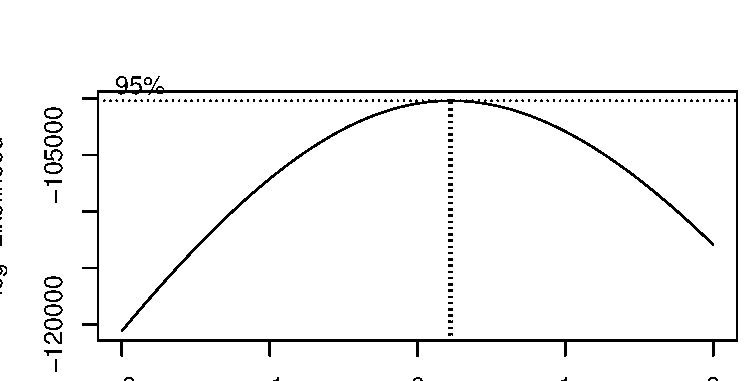
\includegraphics{project_report_files/figure-pdf/unnamed-chunk-7-1.pdf}

}

\end{figure}

\hypertarget{references}{%
\section*{References}\label{references}}
\addcontentsline{toc}{section}{References}

\hypertarget{bibliography-styles}{%
\section{Bibliography styles}\label{bibliography-styles}}

Here are two sample references: \citet{Feynman1963118}
\citet{Dirac1953888}.

By default, natbib will be used with the \texttt{authoryear} style, set
in \texttt{classoption} variable in YAML. You can sets extra options
with \texttt{natbiboptions} variable in YAML header. Example

\begin{verbatim}
natbiboptions: longnamesfirst,angle,semicolon
\end{verbatim}

There are various more specific bibliography styles available at
\url{https://support.stmdocs.in/wiki/index.php?title=Model-wise_bibliographic_style_files}.
To use one of these, add it in the header using, for example,
\texttt{biblio-style:\ model1-num-names}.

\hypertarget{using-csl}{%
\subsection{Using CSL}\label{using-csl}}

If \texttt{cite-method} is set to \texttt{citeproc} in
\texttt{elsevier\_article()}, then pandoc is used for citations instead
of \texttt{natbib}. In this case, the \texttt{csl} option is used to
format the references. By default, this template will provide an
appropriate style, but alternative \texttt{csl} files are available from
\url{https://www.zotero.org/styles?q=elsevier}. These can be downloaded
and stored locally, or the url can be used as in the example header.


  \bibliography{bibliography.bib}


\end{document}
